% !Mode:: "TeX:UTF-8"
% Author: Zhengxi Tian
% Email: zhengxi.tian@hotmail.com

\chapter{研究方法}\label{ch:method}

% 简要说明实验框架。并不复杂,一图足矣。
% 详细说明数据集的统计数据,模型的超参数,训练参数,指标实现的来源,
% 指标的超参数。这些属于Training Procedure或者Experiment的内容。
% 因为是本科毕设,写verbose一些也没关系。
\section{指标测评框架}\label{sec:eval_framework}
我们的实验主要涉及在多个数据集上训练多个模型,然后用多种指标去测量这些系统的句子层面得分和系统层面得分。
表~\ref{tab:experiment_triples}~展示了实验所使用的模型,数据集和指标。
% -- Math & Figure
如图~\ref{fig:framework}~所示,我们的实验首先从让每一个模型$m$和数据集$d$的组合$(m, d) \in M \times D$在训练集上进行训练,
并让训练好的$(m, d)$在测试集上解码产生响应$r$,然后再用每一个指标$s \in S$给$r$在句子层面打分,给$(m, d)$在系统层面打分,
分别得到$\lambda_{u}$和$\lambda_{s}$。
实验的最终结果是一个5元组$(m, d, e, \lambda_{u}, \lambda_{s})$,
表示在数据集$d$上训练的模型$m$在指标$s$的评价下所得的句子层面得分$\lambda_u$和系统层面得分$\lambda_s$。


%本章将详细介绍模型的超参数,训练流程,数据集预处理等实验细节。
\begin{table}[H]
    \centering
    \caption{实验对象一览}
    \label{tab:experiment_triples}
    \begin{tabular}{|r|m{0.6\textwidth}|}
        \hline
        模型 & HRED,LSTM,VHRED \\
        \hline
        数据集 & Ubuntu,OpenSubtitles,LSDSCC \\
        \hline
        指标 & BLEU,ROUGE,METEOR,Vector-Average,
        Vector-Extrema,Greedy-Matching,
        ADEM,PPL,Distinct-N \\
        \hline
    \end{tabular}
\end{table}

\begin{figure}[H]
    \centering
    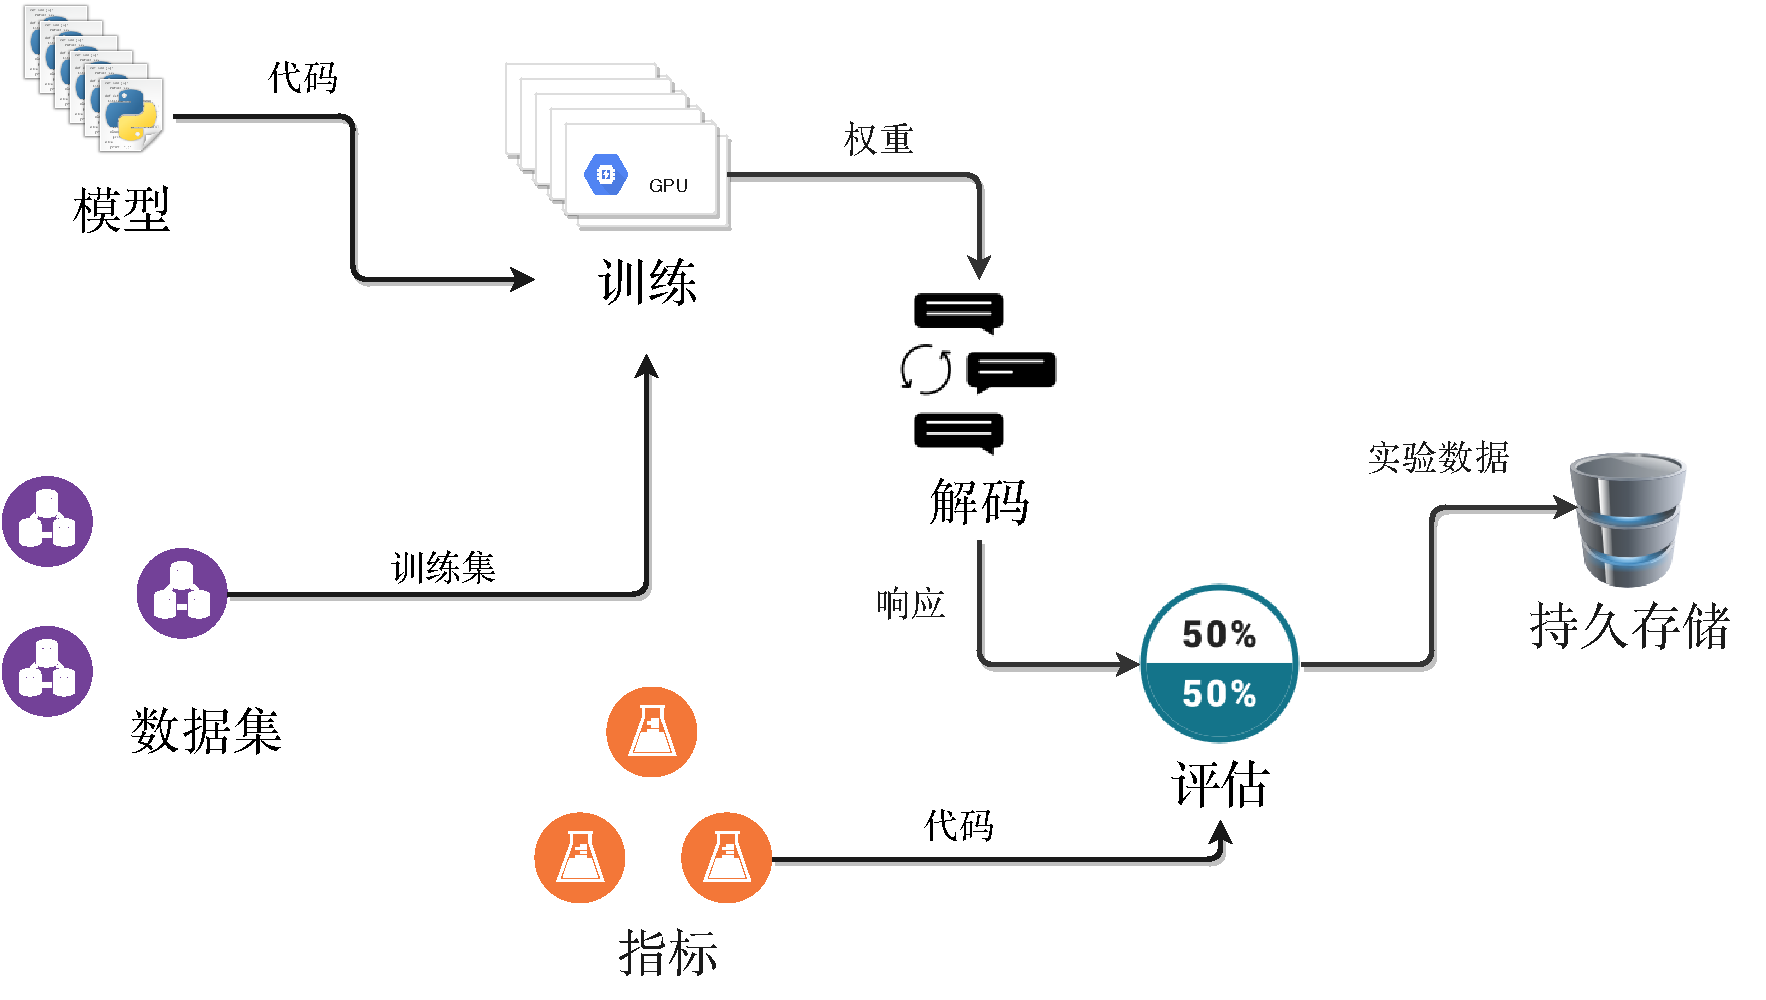
\includegraphics[width=0.8\textwidth]{figure/drawio/eval_v4.pdf}
    \caption{实验框架}
    \label{fig:framework}
\end{figure}

\section{模型超参数设置}\label{sec:model_hparams}
% ------ Model setup ----------- %
在模型超参数方面,我们的设置大致和\cite{VHRED}相同。
我们用Adam\upcite{AdamOpt}来优化所有模型,
一个小批(Mini-batch)处理20个样本。
% -- Dimension of Word Embeddings -- %
我们在Ubuntu上使用维度是300的词嵌入,
在OpenSubtitles和LSDSCC上使用维度是400的词嵌入。
% -- Hidden Units of Utterance Encoder -- %
HRED和VHRED的句子编码器(Utterance Encoder)
在Ubuntu上使用500个隐藏单元,
在OpenSubtitles和LSDSCC上使用1000个隐藏单元
\footnote{LSTM模型是一个语言模型,只有句子解码器。}。
% -- Hidden Units of Context Encoder -- %
HRED和VHRED的上下文编码器(Context Encoder)
在所有数据集上都使用1000个隐藏单元。
% -- Hidden Units of Utterance Decoder -- %
不同模型的句子解码器(Utterance Decoder)
在不同数据集上的隐藏单元数量
如表~\ref{tab:utterance_decoder_hidden_units}~所示。
一般根据数据集的特点来设置不同RNN的隐藏单元数量,
在样本数多或者词汇表大的数据集上训练时,
隐藏单元数量会更多。

\begin{table}[H]
    \centering
    \caption{句子解码器的隐层状态单元数量}
    \label{tab:utterance_decoder_hidden_units}
    \begin{tabular}{llll}
        \toprule
        & HRED & LSTM & VHRED \\
        \midrule
        LSDSCC & 1000 & 2000 & 1000 \\
        OpenSubtitles & 1000 & 2000 & 1000 \\
        Ubuntu & 500 & 2000 & 500 \\
        \bottomrule
    \end{tabular}
\end{table}

% -- Direction of Utterance Encoder -- %
Ubuntu上的模型的句子编码器都使用了单向RNN,
而OpenSubtitles和LSDSCC上的模型的句子编码器则使用双向RNN。
% -- Gate Type of Utterance & Context Encoder -- %
所有模型的句子编码器和上下文编码器(如果有)都使用GRU作为门单元。
% -- Gate Type of Decoder -- %
句子解码器的门单元类型如表~\ref{tab:utterance_decoder_gate_types}~所示
\footnote{OpenSubtitles和LSDSCC上的LSTM模型的解码器都没有使用LSTM门单元,不过它们仍然是语言模型。}。
\begin{table}[H]
    \centering
    \caption{句子解码器的门单元类型}
    \label{tab:utterance_decoder_gate_types}
    \begin{tabular}{llll}
        \toprule
        & HRED & LSTM & VHRED \\
        \midrule
        LSDSCC & LSTM & GRU & GRU \\
        OpenSubtitles & LSTM & GRU & GRU \\
        Ubuntu & LSTM & LSTM & LSTM \\
        \bottomrule
    \end{tabular}
\end{table}

所有的模型都在一台GeForce GTX TITAN X上训练了至少1周。
模型收敛时的困惑度如表~\ref{tab:converged_perplexity}~所示。
\begin{table}[H]
    \centering
    \caption{模型收敛时的困惑度}
    \label{tab:converged_perplexity}
    \begin{tabular}{llll}
        \toprule
        & HRED & LSTM & VHRED \\
        \midrule
        LSDSCC & 32.9229 & 32.5599 & 37.7149 \\
        OpenSubtitles & 41.6392 & 34.2724 & 33.6867 \\
        Ubuntu & 39.1623 & 46.4055 & 40.2486 \\
        \bottomrule
    \end{tabular}
\end{table}

与\cite{VHRED}不同的是,我们没有用预训练的HRED的参数来初始化对应的VHRED。
从实验结果来看,从零开始训练的VHRED也能达到和HRED相匹配的性能。
所有的模型都使用了梯度剪裁,阈值为1。
所有模型在Ubuntu上的学习率为0.0002,
在OpenSubtitles和LSDSCC上的学习率为0.0001。
在解码时,我们使用随机取样。

\section{数据集预处理}
\label{sec:dataset_proprecessing}
我们使用的Ubuntu Dialogue Corpus直接来自Serban等人的项目hed-truncated
\footnote{\url{https://github.com/julianser/hed-dlg-truncated.git}},没有经过任何额外处理。
我们从Li等人的项目Neural-Dialogue-Generation中获取了经过预处理的OpenSubtitles数据
\footnote{\url{https://github.com/jiweil/Neural-Dialogue-Generation.git}}(他们称其为OpenSubData)。
对OpenSubData作了如下处理:
\begin{enumerate}
    \item 将其从整数的下标形式还原为字符串的单词形式;
    \item 将其词汇表文件\texttt{movie\_25000}转化为下标从0开始的
    pickle\footnote{pickle是一个Python特有的序列化格式}格式。
    \item 用Serban等人的\texttt{convert\_text2dict.py}脚本将训练集,测试集和开发集均转换为pickle格式;
    \item 选用OpenSubData中的3轮对话,句子最短长度为6的dialogue3\_6格式作为实际使用的数据集;
    \item 从测试集随机抽取1\%的样本作为正式使用的数据集。
\end{enumerate}

LSDSCC也是一个经过预处理的数据集\footnote{\url{https://drive.google.com/file/d/1nbpbnhwNP14xAc4SAc1 NN5lvEr01dQb/view?usp=sharing}}。
由于它的词汇数量多达50K,为了使内存不至于溢出,我们将其词汇表裁剪至35000个最常见的单词。
此外,由于我们只使用单个参考的指标,因此对LSDSCC的测试集中的多个参考,我们只取第一个参考。
剩下的处理过程类似OpenSubData的处理。

表~\ref{tab:train_set_stats}~是三个数据集的训练集的一些统计数据。
从表中可以看到,OpenSubtitles的样本数量要远远超过其他两个数据集,是Ubuntu的26倍, 是LSDSCC的16倍。
但是,从单词数量来看,OpenSubtitles超过另外两个数据集的倍数却小得多,
这是因为Ubuntu的每一个样本包含了多个句子,其长度要远远超过OpenSubtitles的样本。
这也导致了Ubuntu的样本数量少于LSDSCC,但是单词数量却超过了LSDSCC。
测试集的统计数据如表~\ref{tab:test_set_stats}~所示。
对于LSDSCC的测试集,我们其实可以从其训练集分一部分出来作为测试集,这样可以使样本数量更多。
但是,我们选择了从LSDSCC的多重参考测评集中构造测试集,这导致样本数量只有不到300。

\begin{table}[H]
    \centering
    \caption{训练集的统计数据}
    \label{tab:train_set_stats}
    \begin{tabular}{lllll}
        \toprule
        数据集 & 词汇数量 & 样本数量 & 单词数量 & 轮数 \\
        \midrule
        Ubuntu & 20000 & 448833 & 45697699 & 多轮 \\
        OpenSubtitles & 23876 & 11771393 & 379346841 & 多轮 \\
        LSDSCC & 35008 & 738095 & 32355628 & 单轮 \\
        \bottomrule
    \end{tabular}
\end{table}

\begin{table}[H]
    \centering
    \caption{测试集的统计数据}
    \label{tab:test_set_stats}
    \begin{tabular}{lll}
        \toprule
        数据集 & 样本数量 & 单词数量 \\
        \midrule
        Ubuntu & 18920 & 2045082   \\
        OpenSubtitles & 14714 & 474074 \\
        LSDSCC & 299 & 10914 \\
        \bottomrule
    \end{tabular}
\end{table}

\section{指标配置}\label{sec:metric_config}
我们尽可能使用业界公认的指标实现,并且使用推荐的指标参数。
和\cite{HowNot}一样,我们只考虑单轮对话,并且每个系统输出响应都只有单个参考响应。
% -- BLEU -- %
我们使用NLTK\footnote{\url{https://www.nltk.org/}}提供的BLEU实现, 并且加入了平滑处理。
% -- ROUGE -- %
我们使用了自己实现的ROUGE,并将准确率和召回率的比例设置为1:9,因为在机器翻译领域,
召回率比准确率和人类评价的相关性更高\upcite{METEOR}。
ROUGE-W的权重设置为1.2 。
% -- METEOR -- %
我们使用了METEOR的官方实现\texttt{meteor-1.5.jar},并且按照官方文档
\footnote{\url{http://www.cs.cmu.edu/~alavie/METEOR/README.html}}的说明,
加入对特定语言(英语)的优化过的正则化处理。
% -- PPL -- %
我们使用Serban等人的\texttt{evaluate.py}脚本测量模型的困惑度,
由于该程序对测试样本进行了随机取样,我们无法得知某个样本的确切得分,所以只测得了系统层面的得分。
% -- EB -- %
关于词嵌入的指标,我们对Serban等人的\texttt{embedding\_metrics.py}脚本进行了改写,
使之能测量句子层面的得分;和他们一样,我们使用在谷歌新闻文库(Google News Corpus)上进行训练的
word2vec词嵌入\footnote{\url{https://drive.google.com/file/d/0B7XkCwpI5KDYNlNUTTlSS21pQmM}}。
% -- ADEM -- %
关于ADEM指标,我们使用作者提供的代码库\footnote{\url{https://github.com/mike-n-7/ADEM.git}}和预训练模型
\footnote{\url{https://drive.google.com/file/d/0B-nb1w_dNuMLY0Fad3N1YU9ZOU0/view?usp=sharing}}。
该版本的ADEM使用了VHRED的句子编码器和上下文编码器,并在一个带人类评价的Twitter文库上训练。
我们自己实现了比较简单的Distinct-N指标。
我们的指标还加入了句子长度$\textit{\#words}$,以观察句子长度对不同指标的得分是否有影响。

\section{本章小结}\label{sec:method_conclusion}
本章详细介绍了实验的各项设置,包括模型的超参数和训练过程,
数据集的预处理操作和一些统计数据,以及指标的实现和参数选择。
在下一章中,我们将展示实验的结果并进行讨论。
